\part{Mechanik}
\section{Begrifflichkeiten}
	\subsection{Generalisierte Koordinaten}
		Die generalisierten (oder verallgemeinerten) Koordinaten bilden in der Theoretischen Mechanik und der Technischen Mechanik einen minimalen Satz von unabhängigen Koordinaten zur eindeutigen Beschreibung des räumlichen Zustands des betrachteten Systems. Sie werden so gewählt, dass die mathematische Formulierung von Bewegungen, die Zwangsbedingungen unterliegen, möglichst einfach wird. Z. B. genügt beim mathematischen Pendel statt der x- und z-Koordinate des Massenpunkts die Angabe des Auslenkwinkels, um die Lage eindeutig zu beschreiben. Die konstante Seillänge ist durch die Bindungsgleichung 
		$ l = const $gegeben.
		\begin{figure}[h]
			\centering
			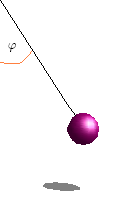
\includegraphics[width=0.15\linewidth]{./pics/me/Pendel}
			\caption{Für das Pendel in der Ebene ergibt sich ein Freiheitsgrad und somit eine generalisierte Koordinate; und zwar $ \phi $}
		\end{figure}
		\leavevmode\\
		Allgemein stimmt die Anzahl der generalisierten Koordinaten, die zur Beschreibung eines Systems mindestens erforderlich sind, mit der Anzahl seiner Freiheitsgrade überein. Die generalisierten Koordinaten spannen den Konfigurationsraum auf.
	\subsection{Arten von Kräften}
		\textbf{Generalisierte Kräfte} sind alle Kräfte die keine Zwangskräfte sind. Sie haben nicht zwangsweise die Einheit der Kraft sondern das Produkt der generalisierte Kraft und zugehöriger generalisierter Koordinate hat die Einheit der Arbeit. So besitzt z.B. die gen. Kraft zu einem Winkel als Koordinate (dimensionslos), die Einheit $ Nm $.\\\\
		\textbf{Zwangskraft} ist beispielsweise die Kraft die vom Untergrund auf einen Klotz wirkt, da er durch die Erdbeschleunigung nach unten gedrückt wird.\\\\
		\textbf{Konservative Kräfte} sind Kräfte die entlang eines geschlossenen Wegintegrals keinerlei Arbeit verrichten. D.h. der Energieinhalt ist am Ende wieder der gleiche. \\\\
		Bei \textbf{Nicht-konservative Kräfte} wird Energie abgeführt (z.B. Reibung). Demnach sind Reibkräfte oder Dämpferkräfte nicht-konservativ. Aber auch Kräfte die Energie in ein System einbringen, wie etwa ein Antriebsdrehmoment sind ebenfalls nicht-konservativ.
	\subsection{Holonome Systeme}
		Ein holonomes System ist in der Mechanik ein System von Körpern, für welches die Lage der Körper über $ n $ generalisierte Koordinaten $ q_{1},q_{2},...,q_{n} $ beschrieben werden kann. Die Koordinaten können entweder vollständig unabhängig voneinander oder über $ m<n $ Zwangsbedingungen miteinander verknüpft sein. 
		\[dim(\bm{q})=dim(DOF)\]
		
		
\section{\textcolor{red}{Kinematik}}
\section{\textcolor{red}{Kinetik}}